\begin{problem}
Доказательство иррациональности $\sqrt{2}$. Доказательство счётности множества $\Q$. Доказательство неполноты множества рациональных чисел.
\end{problem}

\begin{proof} \textbf{Доказательство иррациональности $\sqrt{2}$.}

    Рассмотрим
    уравнение $x^2=2.$ Предположим,
    что у этого уравнения есть
    рациональное решение, т.е.
    $x=\frac{p}{q},$ где дробь
    $\frac{p}{q}$ несократима.
    Тогда $\frac{p^2}{q^2}=2
        \Leftrightarrow p^2=2q^2,$
    откуда следует, что число
    $p^2$ чётное, а тогда и число
    $p$ чётное, т. е. $p=2k,
        k\in\mathbb{Z}.$ Поэтому
    верно равенство $4k^2=2q^2
        \Leftrightarrow 2k^2=q^2,$
    что означает чётность числа
    $q.$ Это означает, что дробь
    $\frac{p}{q}$ сократима
    вопреки нашему предположению.
    Таким образом, число,
    квадрат которого равен
    2, не является рациональным,
    а $x^2=2$ -- это пример уравнения,
    не имеющего решения в рациональных
    числах.
\end{proof}


\begin{proof} \textbf{Доказательство счётности множества $\Q$.}

    Покажем, как присвоить каждому рациональному
    числу свой номер так, чтобы любые два разные
    числа имели разные номера и каждое натуральное
    число являлось номером какого-нибудь
    рационального.

    Назовём высотой рационального числа $\frac{m}{n}$
    величину $h:=|m|+n.$
    Так как дробь неcократима, а $n\in\N,$ то
    при фиксированном $h$ знаменатель $n$ принимает
    не более, чем $h-1$ значение, а при каждом
    фиксированном $n$ для $m$ возможны
    только два варианта $\pm(h-n),$
    поэтому различных рациональных чисел
    с фиксированной высотой $h$ не более, чем
    $2h.$

    Будем нумеровать рациональные
    числа по возрастанию высоты, а при
    фиксированной высоте -- по возрастанию
    самих чисел.
    Число высоты $h=1$ всего одно -- это
    $\frac{0}{1},$ и оно получит номер 1.
    Высоту $h=2$ имеют два рациональных
    числа: $\frac{-1}{1}$ и $\frac{1}{1},$
    они получают номера 2 и 3 соответственно.
    Высота $h=3$ будет у чисел $\frac{-2}{1},
        \frac{-1}{2}, \frac{1}{2}, \frac{2}{1},$
    и эти числа получат номера 4, 5, 6 и 7
    соответственно. Ясно, что между
    натуральными и рациональными
    числами таким образом будет установлено
    взаимно-однозначное соответствие.
\end{proof}

\begin{proof} \textbf{Доказательство неполноты множества рациональных чисел.}

    Пусть
    $A=\{a: a>0, a^2\leq2\},$ а
    $B=\{b: b>0, b^2\geq2\}.$
    Тогда $A$ лежит левее $B,$ т.к.
    для всех $a\in A, b\in B$ имеем
    $0\leq b^2-a^2=(b-a)(b+a),$ откуда,
    в силу того, что $a+b>0,$ следует,
    что $0\leq b-a.$ Докажем,что
    если число $c$ разделяет множества
    $A$ и $B,$ то оно удовлетворяет
    равенству $c^2=2,$  (при этом из примера
    1 будет следовать, что $c$ не является
    рациональным). Предположим противное и
    заметим, что $1\leq c\leq 2$, т. к.
    1 лежит множестве $A,$ а 2 --
    во множестве $B.$

    Возможны два случая. Если $c^2<2,$
    то существуют числа, большие $c,$
    квадрат которых также меньше 2
    (поэтому $c$ не может разделять
    множества $A$ и $B$). Действительно,
    рассмотрим число $c+\frac{2-c^2}{5}.$
    Тогда $\left(c+\frac{2-c^2}{5}\right)^2=
        c^2+2c\frac{2-c^2}{5}+
        \left(\frac{2-c^2}{5}\right)^2<
        c^2+4\frac{2-c^2}{5}+\frac{2-c^2}{5}=2.$
    Таким образом, в этом случае $c$ не
    разделяет наши множества.
    Если же $c^2>2,$ то найдутся числа,
    меньшие $c,$ квадрат которых также
    больше 2. Например, возьмём число
    $c-\frac{c^2-2}{4}.$ При возведении
    его в квадрат получим
    $c^2-2c\frac{c^2-2}{4}+\left(
        \frac{c^2-2}{4}\right)^2>
        c^2-4\frac{c^2-2}{4}=2.$

    Таким образом, если найдётся
    число $c,$ разделяющее множества
    $A$ и $B,$ то обязательно $c^2=2.$
\end{proof}

\newpage
\begin{problem}
Доказательство принципа полноты для множества вещественных чисел. Доказатель-
ство аксиомы Архимеда.
\end{problem}

\begin{theorem}
    На множестве бесконечных
    десятичных дробей выполнен принцип полноты.
\end{theorem}
\begin{proof}
    Пусть подмножество $A$
    множества вещественных чисел
    лежит левее подмножества $B.$
    Если $A$ состоит только из
    неположительных чисел, а $B$ --
    только из неотрицательных, то
    эти множества разделяет 0.

    Если в $A$ есть положительные
    числа, то $B$ состоит только
    из положительных чисел, поэтому
    минимальное значение целой части
    дробей, принадлежащих множеству
    $B,$ не меньше 0. Выберем среди
    всех неотрицательных целых
    чисел, с которых начинаются
    элементы $B,$ минимальное
    и обозначим его через $b_0.$
    Далее рассмотрим все элементы
    множества $B,$ начинающиеся
    с числа $b_0,$ и выберем
    из чисел в первых разрядах
    после запятой минимальный.
    Обозначим его $b_1.$ Теперь
    рассмотрим все элементы множества
    $B,$ начинающиеся с $b_0,b_1,$
    и выберем минимальное из чисел во
    вторых разрядах ($b_3$) и т.д.

    Построим число $c=c_0. c_1c_2c_3
        ...,$ где $c_0=b_0, c_1=b_1$ и
    т. д. По построению $c\leq b$
    для всякого элемента $b$ из
    $B.$

    С другой стороны, если бы нашёлся
    такой элемент $a\in A,$ что
    $c\leq a$  и $c\neq a,$
    то существовал бы разряд
    $k,$ для которого
    $a_k>c_k=b_k,$ и $a_0=c_0=b_0,
        ... ,a_{k-1}=b_{k-1},$ что означало
    бы наличие в $A$ элементов,
    которые больше элементов из $B.$
    Тогда мы бы получили противоречие
    с тем, что $A$ лежит левее $B.$
    Поэтому $a\leq c$ для любого $a\in A,$
    и $c$ разделяет множества $A$ и $B.$

    Если множество $B$ содержит
    отрицательные элементы, то все
    элементы множества $A$ отрицательны.
    Тогда мы рассмотрим
    все неположительные целые
    числа, с которых начинаются
    элементы множества $A,$
    выберем из них максимальный,
    затем выберем все те элементы
    из $A,$ которые начинаются с этого
    максимального и возьмём
    минимальное число в первом разряде
    после запятой у этих элементов и т.д.
    Действуя по аналогии со случаем,
    когда в $A$ есть положительные
    элементы, снова построим число
    $c,$ разделяющее элементы множеств
    $A$ и $B.$ Таким образом, теорема
    доказана.
\end{proof}

\begin{proposition} \textbf{(Аксиома Архимеда).}
    Для любого положительного вещественного числа
    $a$ существует такое натуральное число $n,$ что
    $na\geq1$ (с помощью кванторов: $\forall\;a\in\R\;
        \wedge a>0\exists\;n\in\N:\;na\geq1$).
\end{proposition}
\begin{proof}
    При $a\geq1$ подойдёт $n=1.$ Если $0<a<1,$
    то
    $$
        a=0.\underbrace{0...0}\limits_{k-1 \textrm{ ноль}}
        a_ka_{k+1}...,\;a_k\neq0.
    $$
    Тогда при $n=10^k$ получим
    $10^ka=a_k.a_{k+1}a_{k+2}...\geq1.$
\end{proof}

\newpage
\begin{problem}
Доказательство леммы о вложенных отрезках. Построение вещественной прямой.
\end{problem}

\begin{theorem} \textbf{\textrm{(Лемма о вложенных отрезках)}}
    1) Пусть дана система $M$ вложенных отрезков. Тогда
    существует такое число $c\in\R,$ что для любого отрезка
    $I\in M$ имеем $c\in I,$ то есть все отрезки
    множества $M$ имеют общий элемент $c$.\\
    2) Если множество $M$
    является последовательностью стягивающихся отрезков,
    то элемент $c$ единственен.
\end{theorem}
\begin{proof}
    1) Пусть $A$ и $B$ -- множества левых и правых
    концов отрезков из $M.$ Тогда $a\leq b$ для любых
    $a\in A$ и $b\in B,$ так как либо
    отрезок с левым концом $a$ содержится
    в отрезке с правым концом $b,$ либо наоборот.
    Таким образом, $A$ лежит левее $B,$
    поэтому по принципу полноты существует число
    $c\in\mathbb{R},$ удовлетворяющее
    неравенствам $a\leq c\leq b$
    при всех $a\in\ A, b\in B,$ поэтому
    $c$ принадлежит всем отрезкам из системы $M.$\\
    2) Уже доказано, что
    общая точка $c$ есть. Предположим, что есть
    ещё одна общая точка $c',\;c'< c$
    (если $c'>c,$ то просто переименуем точки).
    Тогда длины всех отрезков не могут
    быть меньше числа $\varepsilon:=c-c'>0,$ что
    противоречит определению последовательности
    стягивающихся отрезков. Поэтому у стягивающихся
    отрезков ровно одна общая точка.
\end{proof}

\begin{center}
    \textsf{Построение вещественной прямой}
\end{center}
Рассмотрим геометрическую интерпретацию
действительных чисел.

Рациональные числа обычно представляют
точками на прямой: отмечается точка ноль,
являющаяся началом отсчёта, а затем
вправо от этой точки откладывают единичный
отрезок, правый конец которого соответствует
числу 1. Любое натуральное число можно
теперь получить, откладывая нужное
число раз единичный отрезок от числа 1
вправо. Разделив единичный отрезок
на $q$ равных частей
(это мы умеем делать, так как
можем получить точку, соответствующую
любому натуральному числу, а тогда можно
на другой прямой отложить натуральное число
$q,$ а затем
воспользоваться теоремой Фалеса) и взяв
одну такую часть, мы получим отрезок длины
$1/q,$ а затем, откладывая такой отрезок
вправо от нуля $p$ раз,
получим точку, соответствующую
обыкновенной дроби $p/q.$ Симметрично
отражая все построенные точки относительно
начала отсчёта, можем получить
точки, соответствующие на прямой
всем рациональным числам.

Построим
на прямой положительное вещественное число
$a=a_0,a_1a_2...$. Для этого сначала
отметим на прямой точку, соответствующую
целому неотрицательному числу $a_0,$ а
затем разобьём отрезок $[a_0, a_0+1]$
на 10 равных частей. После этого
выберем $(a_1+1)$-й отрезок из этих
десяти, разобьем его снова
на 10 равных частей, выберем из
этих новых десяти отрезков $(a_2+1)$-й и т.д..
Построенные отрезки обладают тем свойством,
что любой, построенный на очередном таком шаге,
содержится во всех, построенных на
предыдущих шагах. По лемме о вложенных
отрезках
все эти отрезки имеют единственную общую точку.
Эта точка и соответствует числу $a.$

При такой геометрической интерпретации
можно сказать, что принцип полноты
означает, что при выбранных начале
отсчёта (то есть точке,
соответствующей нулю) и единичном
отрезке любая точка прямой
соответствует единственному действительному
числу, а всякое действительное число
соответствует единственной точке на прямой.
Прямая, точкам которой
поставлены в соответствие действительные
числа, называется \textbf{вещественной прямой}.

\newpage
\begin{problem}
Доказательство единственности предела последовательности. Доказательство ограниченности сходящейся последовательности. Доказательство леммы об отделимости.
\end{problem}

\begin{proposition}
    Пусть у последовательности $\{a_n\}_{n=1}^{\infty}$
    существует предел. Тогда этот предел единственен.
\end{proposition}
\begin{proof}
    От противного: пусть
    $$
        \lim\limits_{n\rightarrow\infty}a_n=A
        \textrm{ и }
        \lim\limits_{n\rightarrow\infty}a_n=B,\;A\neq B.
    $$
    Тогда $|A-B|=\varepsilon_0>0.$ По определению
    предела для  $\varepsilon_0/2$ найдётся
    такой номер $N_1\in\mathbb{N},$
    что при всех $n>N_1$
    имеем $|a_n-A|<\varepsilon_0/2.$
    Для этого же $\varepsilon_0/2$
    найдётся
    такой номер $N_2\in\mathbb{N},$
    что при всех $n>N_2$
    имеем $|a_n-B|<\varepsilon_0/2.$ Тогда
    при $n>\max\{N_1, N_2\},$ применяя
    неравенство треугольника, получим
    $$
        \varepsilon_0=|A-B|=
        |A-a_n+a_n-B|\leq|A-a_n|+|a_n-B|<
        \frac{\varepsilon_0}{2}+\frac{\varepsilon_0}{2}=
        \varepsilon_0.
    $$
    Противоречие.
\end{proof}

\begin{proposition}
    Сходящаяся последовательность ограничена.
\end{proposition}
\begin{proof}
    Обозначим нашу последовательность
    $\{a_n\}_{n=1}^{+\infty}$
    и положим
    $\lim\limits_{n\rightarrow\infty}a_n=A.$
    Тогда из определения предела следует,
    что для $\varepsilon=1$ при всех натуральных
    $n,$ больших некоторого $N\in\mathbb{N},$
    выполнено неравенство $|a_n-A|<1,$
    которое при раскрытии модуля можно
    записать так: $A-1<a_n<A+1.$
    Это значит, что при всех натуральных
    $n>N$ последовательность
    $\{a_n\}_{n=N+1}^{+\infty}$
    ограничена.

    Элементов,
    не входящих в эту последовательность,
    лишь конечное число: $a_1, a_2, ..., a_{N}.$
    Если теперь мы выберем максимальное из
    чисел $|a_1|, |a_2|, ..., |a_{N}|, ... |A-1|$
    и $|A+1|,$
    и обозначим это максимальное значение
    через $M,$ то уже для всех элементов
    последовательности $\{a_n\}_{n=1}^{+\infty}$
    будет выполнено неравенство $|a_n|\leq M,$
    чем и доказана ограниченность.
\end{proof}

\begin{proposition}
    (\textbf{Лемма об отделимости}).
    Пусть $\lim\limits_{n\rightarrow\infty}a_n=A$
    и $A\neq0.$ Тогда существует такое
    натуральное число $N,$ что для всех
    $n>N$ выполнено неравенство
    $|a_n|>\frac{|A|}{2}.$
\end{proposition}

\begin{proof}
    В определении предела
    возьмём $\varepsilon=\frac{|A|}{2}$.
    Для этого $\varepsilon$ по определению
    найдётся такое натуральное число
    $N,$ что при всех
    $n>N\left(\frac{|A|}{2}\right)$ будет
    верно неравенство $|a_n-A|<
        \frac{|A|}{2}.$ По неравенству,
    вытекающему из неравенства треугольника
    (см. лекцию 1) имеем
    $|A|-|a_n|\leq|a_n-A|<\frac{|A|}{2}\Rightarrow
        |A|-\frac{|A|}{2}<|a_n|\Leftrightarrow
        \frac{|A|}{2}<|a_n|.$
    Таким образом, при $N=N\left(\frac{|A|}
        {2}\right)$
    требуемое неравенство выполнено.
\end{proof}

\newpage
\begin{problem}
Доказательство арифметики пределов. Доказательство леммы о зажатом пределе.
\end{problem}

\begin{theorem}(\textbf{Арифметика пределов}).
    Пусть $\lim\limits_{n\rightarrow\infty}a_n=A,$
    $\lim\limits_{n\rightarrow\infty}b_n=B.$ Тогда:\\
    1) $\forall\alpha, \beta\in\mathbb{R}\;\lim\limits_{n\rightarrow\infty}(\alpha a_n
        +\beta b_n)=\alpha\lim\limits_{n\rightarrow\infty}
        a_n+\beta\lim\limits_{n\rightarrow\infty}b_n=
        \alpha A+\beta B;$\\
    2) $\lim\limits_{n\rightarrow\infty}(a_n
        \cdot b_n)=\lim\limits_{n\rightarrow\infty}
        a_n\cdot \lim\limits_{n\rightarrow\infty}b_n=
        A\cdot B;$\\
    3) если $B\neq0,$ $b_n\neq0$ при всех
    натуральных $n,$ то
    $\lim\limits_{n\rightarrow\infty}\frac{a_n}{b_n}
        =\frac{\lim\limits_{n\rightarrow\infty}
            a_n}{\lim\limits_{n\rightarrow\infty}b_n}=
        \frac{A}{B}.$
\end{theorem}
\begin{proof}
    Из определения следует, что $$\forall\varepsilon>0
        \;\exists N_1\;\exists N_2:\;
        \forall n>N_1\;|a_n-A|<\varepsilon \textrm{ и }
        \forall n>N_2\;|b_n-B|<\varepsilon.$$
    Пусть $N=\max\{N_1, N_2\}.$
    Тогда при всех $n>N$ одновременно
    $|a_n-A|<\varepsilon \textrm{ и } |b_n-B|<\varepsilon.$

    Теперь в пункте 1) получаем
    с помощью неравенства
    треугольника при всех $n>N:$
    $|\alpha a_n+\beta b_n-\alpha A-\beta B|
        \leq|\alpha(a_n-A)|+|\beta(b_n-B)|<
        (|\alpha|+|\beta|)\varepsilon.$ Так как
    $\alpha$ и $\beta$ -- фиксированные числа
    по условию, а $\varepsilon$ мы можем
    выбрать сколь угодно малым, то из
    полученного неравенства вытекает
    справедливость первого пункта.

    В пункте 2 получим при всех
    $n>N$: $$|a_nb_n-AB|=|a_nb_n-b_nA+b_nA-AB|\leq
        |b_n(a_n-A)|+|A(b_n-B)|<|b_n|\varepsilon+
        |A|\varepsilon<(M+|A|)\varepsilon.$$
    Здесь число $M$ взято из следующих
    соображений: последовательность
    $\{b_n\}_{n=1}^{+\infty}$ имеет
    предел по условию, поэтому, согласно
    предложению 2, ограничена, а тогда из
    определения ограниченности следует существование
    такого числа $M>0,$ что при всех
    натуральных $n$ $|b_n|<M.$
    Итак, снова $A$ и $M$ фиксированы,
    а $\varepsilon>0$ можно взять
    любым. Из этого следует справедливость
    пункта 2.

    Пункт 3 сведём к пункту 2, пользуясь условием доказываемой
    теоремы
    и леммой об отделимости.
    Мы имеем равенство
    $\lim\limits_{n\rightarrow\infty}\frac{a_n}{b_n}=
        \lim\limits_{n\rightarrow\infty}\left(a_n\cdot
        \frac{1}{b_n}\right),$ поэтому если будет доказано,
    что у последовательности
    $\{\frac{1}{b_n}\}_{n=1}^{+\infty}$ есть предел,
    то получим, в силу пункта 2, что он есть
    и у произведения $a_n\cdot
        \frac{1}{b_n}.$

    Мы докажем даже более
    сильный факт:
    $\lim\limits_{n\rightarrow\infty}\frac{1}{b_n}=
        \frac{1}{B}.$ Действительно, при всех $n>N$ имеем, как
    было написано в начале доказательства, $|b_n-B|<\varepsilon;$
    справедливо также равенство
    $\frac{1}{b_n}-\frac{1}{B}=\frac{|B-b_n|}{|B||b_n|}.$
    Вспоминая, что по лемме отделимости найдётся такое
    натуральное число $N_3,$ что $|b_n|>\frac{|B|}{2},$
    и беря $L=\max\{N, N_3\},$ будем иметь при всех $n>L:$
    $\frac{|B-b_n|}{|B||b_n|}<\frac{|B-b_n|}{|B||
            \frac{|B|}{2}|}<\frac{2}{|B|^2}\varepsilon.$
    (Важно осознать, почему цепочка неравенств
    справедлива!) Таким образом, в силу произвольности
    $\varepsilon,$ мы доказали справедливость
    равенства $\lim\limits_{n\rightarrow\infty}\frac{1}{b_n}=
        \frac{1}{B}.$ Теперь к последовательностям
    $\{a_n\}_{n=1}^{+\infty}$ и $\{\frac{1}{b_n}\}_{n=1}^{+\infty}$
    остаётся применить пункт 2, и третий пункт доказан.
\end{proof}

\begin{theorem} (\textbf{Лемма о зажатом пределе}).
    Пусть
    $\lim\limits_{n\rightarrow\infty}a_n=
        \lim\limits_{n\rightarrow\infty}b_n=A$
    и $a_n\leq c_n\leq b_n,$ начиная
    с некоторого натурального $n.$
    Тогда $\lim\limits_{n\rightarrow\infty}c_n=A.$
\end{theorem}
\begin{proof}
    Из определения следует, что $$\forall\varepsilon>0
        \textrm{ }\exists N_1 \textrm{ и } \exists N_2:
        \forall n>N_1\textrm{ }|a_n-A|<\varepsilon \textrm{ и }
        \forall n>N_2\textrm{ }|b_n-A|<\varepsilon.$$
    Пусть $N=\max\{N_1, N_2\}.$
    Тогда при всех $n>N$ одновременно
    $|a_n-A|<\varepsilon \textrm{ и } |b_n-A|<\varepsilon,$
    поэтому $$A-\varepsilon\leq a_n\leq c_n\leq b_n<
        A+\varepsilon$$ при всех $n>N,$ то есть
    $|c_n-A|<\varepsilon,$ поэтому выполнено
    определение предела для последовательности
    $\{c_n\}_{n=1}^{\infty}.$
\end{proof}

\newpage
\begin{problem}
Доказательство существования точной верхней и нижней граней ограниченного множества. Доказательство теоремы Вейерштрасса для последовательностей.
\end{problem}

\begin{theorem}
    Пусть множество $A$ непусто и ограничено
    сверху. Тогда существует $\sup A.$
\end{theorem}
\begin{proof}
    Пусть $B$ -- множество всех верхних граней
    множество $A.$ Оно непусто, так как множество
    $A$ ограничено сверху по условию. Из
    определения ограниченности сверху вытекает,
    что $A$ левее $B.$ По принципу полноты
    существует $c\in\mathbb{R},$ разделяющее
    множества $A$ и $B$. По определению
    разделяющего элемента $$a\leq c\leq b
        \textrm{ при всех } a\in A, b\in B.$$ В частности,
    отсюда следует, что $c$ -- наименьшая
    из верхних граней, то есть, по определению,
    точная верхняя грань.
\end{proof}

\begin{theorem} \textrm{(Вейерштрасс)}.
    Монотонная и ограниченная последовательность
    имеет предел.
\end{theorem}
\begin{proof}
    Будем считать (без ограничения общности),
    что последовательность
    $\{a_n\}_{n=1}^{+\infty}$ неубывающая
    и $A=\{a_1, a_2, a_3...\}$ -- множество
    значений этой последовательности.
    Тогда по условию она ограничена сверху,
    поэтому по теореме 1 существует точная
    верхняя грань множества значений $a=\sup A$.

    Докажем, что
    $\lim\limits_{n\rightarrow\infty}a_n=a.$
    По второму определению точной верхней
    грани
    $$
        \forall\varepsilon>0\;\exists
        a_k\in A:\;a_k>a-\varepsilon
        \textrm{ и }
        \forall
        n\in\mathbb{N}\;a_n\leq a<a+\varepsilon.
    $$
    Так как последовательность монотонна,
    при всех $n>k$ $a_k\leq a_n,$
    поэтому $a_n>a-\varepsilon.$
    Таким образом, доказано, что
    для всякого $\varepsilon>0$
    можно взять такое натуральное число $k,$
    что для всех $n>k$ $a-\varepsilon<a_n<
        a+\varepsilon\Leftrightarrow
        |a_n-a|<\varepsilon,$ то есть
    для последовательности
    $\{a_n\}_{n=1}^{+\infty}$ выполнено
    определение предела.

    Если последовательность $\{a_n\}_{n=1}^{+\infty}$
    невозрастающая, то для неубывающей последовательности
    $\{-a_n\}_{n=1}^{+\infty}$ наличие предела
    доказывается, как и выше, а тогда существование
    предела у $\{a_n\}_{n=1}^{+\infty}$ следует
    из арифметики предела.
\end{proof}

\newpage
\begin{problem}
Итерационная формула Герона (Пример 2, Лекция 4). Доказательство существования предела последовательности $a_n = \left(1+\frac{1}{n}\right)^n$
\end{problem}

Покажем, как можно вычислять
приближённое значение корня
заданного числа $a$ с помощью
\textbf{итерационной формулы Герона}.
Пусть $$a_1=a>0, \ a_{n+1}=
    \frac{1}{2}\left(a_n
    +\frac{a}{a_n}\right).$$
Требуется найти
$\lim\limits_{n\rightarrow\infty}a_n.$
Предположим, что предел
этой последовательности
существует и равен $A.$
Из неравенства между средним
арифметическим и средним геометрическим
будем иметь: $a_{n+1}=
    \frac{1}{2}\left(a_n
    +\frac{a}{a_n}\right)\geq
    \frac{1}{2}\sqrt{a_n
        \cdot\frac{a}{a_n}}=\sqrt{a}.$
Тогда $A\neq0$ и мы можем перейти к пределу
в равенстве $a_{n+1}=
    \frac{1}{2}\left(a_n
    +\frac{a}{a_n}\right).$
Пользуясь арифметикой пределов,
будем иметь:
$$
    A=\lim\limits_{n\rightarrow\infty}a_{n+1}=
    \frac{1}{2}\left(\lim\limits_{n\rightarrow\infty}a_n
    +\frac{a}{\lim\limits_{n\rightarrow\infty}a_n}\right)=
    \frac{1}{2}\left(A
    +\frac{a}{A}\right)\\
    \Leftrightarrow A^2=a \Leftrightarrow A=\pm\sqrt{a},
$$
откуда получим $A=\sqrt{a},$ так как $A\geq
    \sqrt{a}$ по теореме о переходе к
пределу в неравенствах.

Теперь необходимо доказать, что
наше предположение оправдано, то есть
предел последовательности существует.
Мы уже доказали, что последовательность
ограничена снизу, поэтому если будет
доказано, что она не возрастает, то
существование предела будет следовать
из теоремы Вейерштрасса. Имеем:
$$
    a_{n+1}=
    \frac{1}{2}\left(a_n
    +\frac{a}{a_n}\right)\leq
    \frac{1}{2}\left(a_n
    +\frac{a_n^2}{a_n}\right)=a_n,
$$
чем и доказано, что последовательность
не возрастает.

\begin{theorem}
    Последовательность $a_n=\left(1+\frac{1}{n}\right)^n$
    имеет предел.
\end{theorem}
\begin{proof}
    Докажем, что эта последовательность
    монотонно возрастает и ограничена
    сверху. Тогда существование предела
    будет следовать из теоремы Вейерштрасса.\\
    {\bf Ограниченность.} По биному Ньютона
    имеем:
    \begin{multline*}
        a_n=\left(1+\frac{1}{n}\right)^n=C_n^0\left(\frac{1}{n}\right)^0+
        C_n^1\left(\frac{1}{n}\right)^1+C_n^2\left(\frac{1}{n}\right)^2+
        ...+C_n^{n-1}\left(\frac{1}{n}\right)^{n-1}+
        C_n^n\left(\frac{1}{n}\right)^n=\\
        =1+1+\frac{1}{2!}\frac{n\cdot(n-1)}{n^2}+
        \frac{1}{3!}\frac{n\cdot(n-1)\cdot(n-2)}{n^3}+...+
        \frac{1}{(n-1)!}\frac{n\cdot(n-1)\cdot...\cdot2}{n^{n-1}}+\\
        +\frac{1}{n!}\frac{n\cdot(n-1)\cdot...\cdot2\cdot1}{n^n}=
        2+\sum\limits_{k=2}\limits^{n}\frac{1}{k!}
        \left(1-\frac{1}{n}\right)\cdot...\cdot\left(1-\frac{k-1}{n}\right)
    \end{multline*}
    (обязательно разберитесь, как получаются друг из друга
    эти равенства).

    Теперь отметим, что $\frac{1}{k!}
        \left(1-\frac{1}{n}\right)\cdot...
        \cdot\left(1-\frac{k-1}{n}\right)\leq\frac{1}{k!}
        =\frac{1}{1\cdot2\cdot3\cdot...\cdot(k-1)\cdot k}
        \leq\frac{1}{2^{k-1}},$ откуда получим, что
    $a_n\leq 2+\sum\limits_{k=2}\limits^{n}\frac{1}{2^{k-1}}=
        3-\frac{1}{2^{n-1}}<3.$\\
    {\bf Монотонность.} Отметим, что
    $\left(1-\frac{1}{n}\right)\cdot...\cdot
        \left(1-\frac{k-1}{n}\right)\leq
        \left(1-\frac{1}{n+1}\right)\cdot...
        \cdot\left(1-\frac{k-1}{n+1}\right)$
    Таким образом, имеем цепочку неравенств:
    \begin{multline*}
        a_n=2+\sum\limits_{k=2}\limits^{n}\frac{1}{k!}
        \left(1-\frac{1}{n}\right)\cdot...\cdot\left(1-\frac{k-1}{n}\right)
        \leq2+\sum\limits_{k=2}\limits^{n}\frac{1}{k!}
        \left(1-\frac{1}{n+1}\right)\cdot...\cdot\left(1-\frac{k-1}{n+1}\right)\leq\\
        \leq2+\sum\limits_{k=2}\limits^{n+1}\frac{1}{k!}
        \left(1-\frac{1}{n+1}\right)\cdot...\cdot\left(1-\frac{k-1}{n+1}\right)=a_{n+1}
    \end{multline*}
    (почему верно последнее неравенство?).

    Итак, доказаны ограниченность сверху и монотонное
    возрастание последовательности, поэтому она имеет
    предел.
\end{proof}

\newpage
\begin{problem}
Доказательство теоремы Больцано – Вейерштрасса. Критерий существования предела последовательности в терминах частичных пределов.
\end{problem}

\begin{theorem}\textbf{(Больцано -- Вейерштрасс.)}
    Из всякой ограниченной последовательности
    можно выбрать сходящуюся подпоследовательность.
\end{theorem}
\begin{proof}
    Если последовательность $\{a_n\}_{n=1}^{\infty}$
    ограничена, то
    $$
        \exists C>0:\;\forall n\in\N\;|a_n|<C,
    $$
    то есть все элементы последовательности
    содержатся в отрезке $[-C, C].$
    Разделим этот отрезок пополам.
    Хотя бы в одном из получившихся отрезков
    содержится бесконечно много
    элементов последовательности. Выберем
    отрезок, в котором содержится бесконечно
    много элементов и назовём его $I_1$
    (если бесконечно много элементов в обеих
    половинах, то выберем любую).
    Выберем какой-либо элемент $a_{n_1}\in I_1$
    и положим $b_1=a_{n_1}.$ Разобьём отрезок
    $I_1$ пополам и выберем ту его половину,
    в которой содержится бесконечно много
    элементов последовательности. Назовём
    его $I_2$ и выберем $a_{n_2}\in I_2$ так,
    чтобы $n_2$ было больше $n_1,$ и положим
    $a_{n_2}=b_2.$ Затем разобьём отрезок $I_2$
    пополам, выберем ту половину $I_3,$ в которой
    содержится бесконечно много элементов
    последовательности, возьмём элемент
    $a_{n_3}\in I_3,$ причём $n_3>n_2,$
    и обозначим $b_3=a_{n_3}.$ Продолжая этот
    процесс, построим последовательность
    вложенных отрезков $\{I_k\}_{k=1}^{\infty}$
    и последовательность $\{b_k\}_{k=1}^{\infty},$
    причём $b_k\in I_k$ и $\{b_k\}_{k=1}^{\infty}$
    является подпоследовательностью последовательности
    $\{a_n\}_{n=1}^{\infty}.$

    При этом $|I_k|=\frac{2C}{2^k}\rightarrow0,\;n
        \rightarrow+\infty,$ поэтому последовательность
    отрезков $\{I_k\}_{k=1}^{\infty}$ является
    стягивающейся и имеет единственную
    общую точку $b,$ причём для любого
    $\varepsilon>0$ при всех достаточно
    больших $k$ выполнены неравенства
    $$
        |b_k-b|\leq\frac{C}{2^{k-1}}<\frac{C}{2^{k-2}}
        <\varepsilon,
    $$
    поэтому $\lim\limits_{k\rightarrow\infty}
        b_{k}=b.$
    Таким образом, мы выбрали подпоследовательность
    последовательности $\{a_n\}_{n=1}^{\infty},$
    имеющую предел.
\end{proof}

\begin{theorem}
    Ограниченная последовательность имеет предел
    тогда и только тогда, когда у неё только
    один частичный предел.
\end{theorem}
\begin{proof}
    \emph{Необходимость}
    этого условия -- это предложение 2.

    Докажем \emph{достаточность}.
    Пусть $a$ -- единственный частичный предел
    последовательности $\{a_n\}_{n=1}^{\infty}.$
    Тогда, по теореме 1,
    $\lowlim\limits_{n\rightarrow\infty}a_n=
        \uplim\limits_{n\rightarrow\infty}a_n=a.$
    По определению верхнего и нижнего предела
    и теореме о зажатом пределе из неравенств
    $m_{n-1}\leq a_n\leq M_{n-1}$
    получаем, что $\lim\limits_{n\rightarrow\infty}
        a_n=a.$
\end{proof}

\newpage
\begin{problem}
Доказательство того, что верхний и нижний пределы являются частичными пределами.
\end{problem}

\begin{theorem}
    Если последовательность $\{a_n\}_{n=1}^{\infty}$
    ограничена, то $\uplim\limits_{n\rightarrow\infty}a_n$
    и $\lowlim\limits_{n\rightarrow\infty}a_n$ являются
    частичными пределами этой последовательности
    и все частичные пределы
    последовательности $\{a_n\}_{n=1}^{\infty}$
    принадлежат отрезку
    $[\lowlim\limits_{n\rightarrow\infty}a_n,
                \uplim\limits_{n\rightarrow\infty}a_n].$
\end{theorem}
\begin{proof}
    Нам необходимо построить подпоследовательность,
    предел которой равен
    $M:=\uplim\limits_{n\rightarrow\infty}a_n.$
    Построим эту подпоследовательность так:
    на первом шаге выберем элемент $a_{n_1},$
    удовлетворяющий условиям
    $$M_{1}-1<a_{n_1}\leq M_{1}.$$
    Это возможно
    в силу определения точной верхней грани, так
    как $M_1-1$ уже не является точной
    верхней гранью для множества
    $
        \{a_{2}, \ a_{3}, \ ...\},
    $
    а поэтому найдётся нужный элемент.

    Элемент $a_{n_2}$ должен быть таким
    элементом исходной последовательности
    $\{a_n\},$ что $n_2>n_1.$
    Выберем его так, чтобы он удовлетворял
    неравенствам
    $$M_{n_1}-1/2<a_{n_2}\leq M_{n_1}.$$
    Элемент, удовлетворяющий таким условиям,
    найдётся снова по определению точной
    верхней грани, а неравенство
    $n_2>n_1$ выполнено, так как согласно
    определению $M_{n_1}$ элемент $a_{n_2}$
    выбирается из множества
    $
        \{a_{n_1+1}, \ a_{n_2+2}, \ ...\},
    $
    в котором все элементы с номерами,
    большими $n_1.$

    Продолжая этот процесс,
    мы на $m+1$-м шаге получим элемент $a_{n_{m+1}},$
    удовлетворяющий неравенствам
    $$M_{n_{m}}-\frac{1}{m+1}<
        a_{n_{m+1}}\leq M_{n_{m}}.$$ При этом
    $n_1<n_2<n_3<...<n_{m+1}<... .$
    По определению верхнего предела,
    $$\lim\limits_{n\rightarrow+\infty}M_n:=M,$$ а тогда
    и любая подпоследовательность
    последовательности $\{M_n\}_{n=1}^{\infty}$
    сходится к тому же пределу.
    Таким образом имеем равенства:
    $$M=\lim\limits_{k\rightarrow+\infty}M_{n_k}=
        \lim\limits_{k\rightarrow+\infty}
        \left(M_{n_{k}}-\frac{1}{k+1}\right).$$
    Тогда, по лемме о зажатом пределе,
    $M=\lim\limits_{k\rightarrow+\infty}a_{n_k},$
    то есть верхний предел является
    частичным пределом последовательности.
    Доказательство для нижнего предела
    полностью аналогично.

    Докажем теперь, что любой частичный
    предел $a$ лежит на отрезке
    $[\lowlim\limits_{n\rightarrow\infty}a_n,
                \uplim\limits_{n\rightarrow\infty}a_n].$
    По определению найдётся подпоследовательность
    $\{a_{n_l}\}_{l=1}^{\infty},$ которая
    сходится к $a.$ Тогда $m_{n_{l-1}}\leq
        a_{n_l}\leq M_{n_{l-1}},$ поэтому по теореме
    о предельном переходе в неравенствах будем
    иметь
    $\lowlim\limits_{n\rightarrow\infty}a_n
        \leq a\leq
        \uplim\limits_{n\rightarrow\infty}a_n.$
\end{proof}

\newpage
\begin{problem}
Доказательство критерия Коши для последовательностей.
\end{problem}

\begin{theorem}
    Последовательность $\{a_n\}_{n=1}^{\infty}$
    имеет предел \textbf{тогда и только
        тогда}, когда она фундаментальна.
\end{theorem}
Выделенная жирным шрифтом фраза как
раз и означает, что теорема является
критерием. Из достаточности
следует, что \textbf{мы можем
    выяснить, что у последовательности
    существует предел, не вычисляя этот
    предел непосредственно.} Существуют
последовательности, где нахождение
предела является гораздо более
сложной задачей, чем проверка
фундаментальности последовательности.
Особенно хорошо это будет видно,
когда мы начнём изучать бесконечные
суммы, то есть ряды. Перейдём к доказательству.
\begin{proof}
    \textbf{Необходимость.} Итак, дано, что есть
    предел, то есть
    $\lim\limits_{n\rightarrow\infty}a_n=A.$
    Нужно доказать, что последовательность
    $\{a_n\}_{n=1}^{\infty}$ фундаментальна.
    Для этого выберем такое $\varepsilon>0,$
    что, начиная с некоторого номера
    $N\in\mathbb{N},$ при всех
    $n>N$
    выполнено неравенство $|a_n-A|<
        \frac{\varepsilon}{2}.$ Тогда при любых
    $n, m>N$ имеем:
    $|a_n-a_m|\leq |a_n-A|+|a_m-A|<
        \frac{\varepsilon}{2}+\frac{\varepsilon}{2}
        <\varepsilon,$ то есть
    $\{a_n\}_{n=1}^{\infty}$ удовлетворяет
    определению фундаментальной последовательности.

    \textbf{Достаточность.} Дано, что
    последовательность $\{a_n\}_{n=1}^{\infty}$
    фундаментальна. Требуется доказать, что у неё
    есть предел.

    Покажем, что последовательность ограничена.
    Действительно, при $\varepsilon=1$ найдётся
    такое натуральное $N,$ что при
    $n=N+1, m>N$ выполнено неравенство
    $|a_m-a_{N+1}|<1,$ а это равносильно тому, что
    $a_{N+1}-1<a_m<a_{N+1}+1.$ Так как
    $N$ -- фиксированное число, то можно
    утверждать, что, начиная с номера
    $N+1,$ наша последовательность
    принадлежит интервалу
    $(a_{N+1}-1, a_{N+1}+1),$ то есть
    является ограниченной.
    За пределами интервала могут лежать
    только числа $a_1, a_2,
        a_3, ..., a_N.$
    Тогда при всех натуральных
    $n$ имеем $$a_n\leq\max\{a_1, a_2,
        a_3, ..., a_{N+1}+1\}\textrm{ и }
        a_n\geq\min\{a_1, a_2,
        a_3, ..., a_{N+1}-1\}.$$ Таким образом,
    ограниченность доказана.

    Тогда, в силу леммы Больцано -- Вейерштрасса
    найдётся сходящаяся подпоследовательность
    $b_k=a_{n_k}$ последовательности
    $\{a_n\}_{n=1}^{\infty}.$ Обозначим
    её предел через $A.$

    Для любого $\varepsilon>0$ существует
    такое $N_1\in\mathbb{N},$
    что при всех $k>N_1$ $|b_k-A|<\varepsilon.$
    Для этого же $\varepsilon>0$ существует
    такое $N_2\in\mathbb{N},$
    что при всех $n, m>N_2$ $|a_n-a_m|<
        \varepsilon.$ Пусть
    $M:=\max\{N_1, N_2\},$ тогда
    при всех
    $n>M$ и $k>M$ имеем $n_k>M$
    (объясните, почему!) и
    $$
        |a_n-A|\leq|a_n-a_{n_k}|+|a_{n_k}-A|<
        \varepsilon+\varepsilon=2\varepsilon,
    $$
    что в силу произвольности $\varepsilon>0$
    доказывает равенство
    $\lim\limits_{n\rightarrow\infty}a_n=A.$
\end{proof}

\newpage
\begin{problem}
Доказательство расходимости последовательности $a_n = 1 + \frac{1}{2} + \frac{1}{3} + \dots + \frac{1}{n}$ (Пример 2, Лекция 6). Доказательство критерия Коши сходимости ряда. Доказательство необходимого признака сходимости ряда. Связь абсолютной сходимости ряда со сходимостью  (Предложение 2, Лекция 7).
\end{problem}

\begin{proof} \textbf{Расходимость гармонического ряда.}

    Рассмотрим теперь последовательность
    $a_n=1+\frac{1}{2}+\frac{1}{3}+...+\frac{1}{n}.$
    Докажем, что она не является фундаментальной.
    Для этого нужно доказать, что
    при некотором $\varepsilon>0$ для любого
    натурального $N$ найдутся такие натуральные
    $m, n>N,$ что $|a_m-a_n|\geq\varepsilon.$
    Действительно, пусть задано натуральное
    $N.$ Возьмём $n=N+1,\;m=2N+2=2n.$ Тогда
    получим:
    \begin{multline*}
        |a_{2n}-a_n|=\left|1+\frac{1}{2}+...+\frac{1}{n}+
        ...+\frac{1}{2n}-1-\frac{1}{2}-...-\frac{1}{n}\right|
        =\left|\frac{1}{n+1}+...+\frac{1}{n+2}+
        ...+\frac{1}{2n}\right|\geq\\
        \geq\underbrace{\left|\frac{1}{2n}+...+\frac{1}{2n}\right|}
        \limits_{n \textrm{ слагаемых}}
        =\frac{n}{2n}=\frac{1}{2}.
    \end{multline*}
    Таким образом, для любого натурального $N$
    найдутся два таких номера $m, n>N,$
    что $|a_m-a_n|\geq\frac{1}{2},$ то есть
    последовательность не является фундаментальной,
    поэтому у неё нет предела.
\end{proof}

\begin{theorem} \textbf{(Критерий Коши сходимости ряда.)}
    Ряд $\sum\limits_{n=1}\limits^{\infty}a_n$ сходится тогда
    и только тогда, когда для любого числа $\varepsilon>0$
    существует такое натуральное число $N,$ что
    при любом $n>N$ и любом $p\in\mathbb{N}$
    выполнено неравенство $|a_{n+1}+...+a_{n+p}|<\varepsilon.$
\end{theorem}

\begin{proof}

    Рассмотрим критерий Коши в применении именно к рядам,
    а точнее -- к последовательности частичных сумм.
    Напомним, что в критерии Коши фигурирует
    неравенство $|a_n-a_m|<\varepsilon$. Рассмотрим
    последовательность частичных сумм
    $\{S_n\}_{n=1}^{\infty}$ некоторого ряда.
    Пусть $m>n.$ Тогда $m=n+p$ для некоторого
    натурального $p.$  Неравенство из критерия
    Коши перепишется в виде:
    $$
        |S_m-S_n|=|a_1+a_2+a_3+...+a_{n-1}+a_{n}+a_{n+1}+...+a_{n+p}-
        (a_1+a_2+...+a_n)|=|a_{n+1}+...+a_{n+p}|<\varepsilon.
    $$
\end{proof}

\begin{proposition}\textbf{(Необходимый признак сходимости ряда).}
    Пусть ряд $\sum\limits_{n=1}\limits^{\infty}a_n$
    сходится. Тогда $\lim\limits_{n\rightarrow\infty}
        a_n=0.$
\end{proposition}
\begin{proof}
    Сходимость ряда -- это по определению
    наличие предела у последовательности
    частичных сумм $\{S_n\}_{n=1}^{\infty}.$
    Пусть $S=\lim\limits_{n\rightarrow\infty}S_n.$
    Тогда $S=\lim\limits_{n\rightarrow\infty}S_{n-1},$
    (отбрасывание $S_1$ не влияет на сходимость)
    и по арифметике предела, получим
    $$\lim\limits_{n\rightarrow\infty}
        a_n=\lim\limits_{n\rightarrow\infty}(S_{n}-S_{n-1})=
        \lim\limits_{n\rightarrow\infty}S_{n}-
        \lim\limits_{n\rightarrow\infty}S_{n-1}=S-S=0.$$
\end{proof}

\begin{proposition}
    Из сходимости ряда
    $\sum\limits_{n=1}\limits^{\infty}|a_n|$
    следует сходимость ряда
    $\sum\limits_{n=1}\limits^{\infty}a_n.$
\end{proposition}
\begin{proof}
    Из сходимости ряда
    $\sum\limits_{n=1}\limits^{\infty}|a_n|$
    следует справедливость критерия Коши:
    $$\forall\varepsilon>0 \ \exists N\in
        \mathbb{N}: \ \forall n>N\wedge
        p\in\mathbb{N} \ |a_{n+1}|+...+|a_{n+p}|<\varepsilon.$$
    Из неравенства треугольника следует,
    что $|a_{n+1}+...+a_{n+p}|\leq|a_{n+1}|+...+|a_{n+p}|,$
    то есть для ряда $\sum\limits_{n=1}\limits^{\infty}a_n$
    выполнен критерий Коши, поэтому он сходится.
\end{proof}

\newpage
\begin{problem}
Доказательство критерия сходимости рядов с неотрицательными членами. Доказательство признака сравнения. Доказательство признака сравнения в предельной форме.
\end{problem}

\begin{proposition}
    Если $a_n\geq0$ $\forall n\in\mathbb{N},$
    то ряд $\sum\limits_{n=1}\limits^{\infty}a_n$
    сходится тогда и только тогда,
    когда ограничена последовательность его
    частичных сумм.
\end{proposition}
\begin{proof}
    Так как все элементы ряда неотрицательны, то
    имеем:
    $$S_{n+1}-S_n=a_{n+1}\geq0\;\Leftrightarrow\;
        S_{n+1}\geq S_n,$$ поэтому последовательность
    частичных сумм $\{S_n\}_{n=1}^{\infty}$
    не убывает. Из того, что она ограничена,
    следует, по теореме Вейерштрасса, что у неё
    есть предел, то есть ряд сходится по
    определению.

    Обратно, если у ряд сходится, то
    последовательность
    частичных сумм сходится, а тогда она
    она ограничена, так как сходящаяся
    последовательность ограничена,
    что уже было доказано в прошлых
    лекциях.
\end{proof}

\begin{theorem} \textbf{(Признак сравнения).}
    Пусть при всех натуральных $n,$
    начиная с некоторого номера,
    выполнены неравенства $0\leq a_n
        \leq b_n.$ Тогда из сходимости
    ряда $\sum\limits_{n=1}\limits^{\infty}b_n$
    следует сходимость ряда
    $\sum\limits_{n=1}\limits^{\infty}a_n,$
    а из расходимости ряда
    $\sum\limits_{n=1}\limits^{\infty}a_n$
    следует расходимость ряда
    $\sum\limits_{n=1}\limits^{\infty}b_n.$
\end{theorem}
\begin{proof}
    Так как любое конечное число
    элементов не влияет на сходимость,
    то будем считать, что условия
    выполнены уже при $n=1.$
    Тогда $$A_n=a_1+a_2+...+a_n\leq
        b_1+b_2+...+b_3=B_n$$
    при всех натуральных $n.$
    В силу предыдущего предложения,
    если сходится ряд
    $\sum\limits_{n=1}\limits^{\infty}b_n,$
    то последовательность его частичных
    сумм $\{B_n\}_{n=1}^{\infty}$
    ограничена, а тогда ограничена
    и последовательность частичных
    сумм $\{A_n\}_{n=1}^{\infty}$
    (например, тем же числом, что
    элементы последовательности $\{B_n\}$),
    поэтому, опять-таки в силу
    предложения 3, сходится ряд
    $\sum\limits_{n=1}\limits^{\infty}a_n.$
    Если же расходится ряд
    $\sum\limits_{n=1}\limits^{\infty}a_n,$
    то его последовательность частичных
    сумм $\{A_n\}_{n=1}^{\infty}$
    не является ограниченной, поэтому
    неограничена последовательность
    $\{B_n\}_{n=1}^{\infty},$
    а тогда и ряд
    $\sum\limits_{n=1}\limits^{\infty}b_n$
    расходится.
\end{proof}

\begin{proposition} \textbf{(Признак сравнения в предельной форме).}
    Пусть при всех натуральных $n,$
    начиная с некоторого числа $N\in\N$,
    выполнены неравенства $a_n\geq0,\;b_n>0,$
    а также
    $\lim\limits_{n\rightarrow+\infty}\frac{a_n}{b_n}=A,$
    причём $A\in(0, +\infty).$
    Тогда ряды $\sum\limits_{n=1}\limits^{\infty}b_n$
    и $\sum\limits_{n=1}\limits^{\infty}a_n$
    или оба сходятся, или оба расходятся.
\end{proposition}
\begin{proof}
    Так как любое конечное число
    элементов не влияет на сходимость,
    то будем считать, что условия
    выполнены уже при $N=1.$
    Пусть $\varepsilon=\frac{A}{2}.$
    Тогда найдётся такое $N_1\in\N,$
    что при всех $n>N_1$ $|\frac{a_n}{b_n}-
        A|<\frac{A}{2},$
    откуда получаем
    $$
        \frac{A}{2}b_n<a_n<\frac{3A}{2}b_n.
    $$
    Таким образом, если сходится ряд
    $\sum\limits_{n=1}\limits^{\infty}b_n$,
    то сходится и ряд
    $\sum\limits_{n=1}\limits^{\infty}\frac{3A}{2}b_n$
    (это следует из определения сходимости и арифметики
    пределов),
    а тогда по признаку сравнения сходится и ряд
    $\sum\limits_{n=1}\limits^{\infty}a_n,$
    а если расходится ряд
    $\sum\limits_{n=1}\limits^{\infty}b_n,$ то
    вместе с ним расходится ряд
    $\sum\limits_{n=1}\limits^{\infty}\frac{A}{2}b_n,$
    а тогда по признаку сравнения расходится ряд
    $\sum\limits_{n=1}\limits^{\infty}a_n.$
\end{proof}

\newpage
\begin{problem}
Доказательство мажорантного признака Вейерштрасса. Доказательство признака разрежения Коши. Исследование на сходимость ряда $\sum_{n=1}^{\infty} \frac{1}{n^p}$ (Пример 2, Лекция 8).
\end{problem}

\begin{proposition} \textbf{(Мажорантный признак Вейерштрасса).}
    Пусть при всех натуральных $n,$
    начиная с некоторого числа $N\in\N$,
    выполнены неравенства $b_n\geq|a_n|$
    и ряд $\sum\limits_{n=1}\limits^{\infty}b_n$
    сходится. Тогда ряд
    $\sum\limits_{n=1}\limits^{\infty}a_n$
    сходится.
\end{proposition}
\begin{proof}
    По признаку сравнения ряд
    $\sum\limits_{n=1}\limits^{\infty}|a_n|$
    сходится, то есть ряд
    $\sum\limits_{n=1}\limits^{\infty}a_n$ сходится
    абсолютно. Как мы уже знаем, если ряд сходится
    абсолютно, то он сходится.
\end{proof}

\begin{theorem}\textbf{(Признак разрежения Коши).}
    Если последовательность
    $\{a_n\}_{n=1}^{\infty}$ не возрастает
    и $a_n\geq0$ при любом натуральном
    $n,$ то ряд
    $\sum\limits_{n=1}\limits^{+\infty}a_n$
    сходится тогда и только тогда, когда
    сходится ряд
    $\sum\limits_{n=1}\limits^{\infty}2^na_{2^n}.$
\end{theorem}
\begin{proof}
    В силу того, что последовательность
    $\{a_n\}_{n=1}^{+\infty}$
    не возрастает и отбрасывание первого
    элемента не влияет на сходимость,
    имеем неравенства
    \begin{multline*}
        a_2+2a_4+4a_8+...+2^{n-1}a_{2^{n}}
        \leq a_2+a_3+a_4+a_5+a_6+a_7+a_8+...+a_{2^n}\leq
        2a_2+4a_4+8a_8+...+2^na_{2^n}.
    \end{multline*}
    Таким образом ограниченность частичных
    сумм одного из рядов в условии равносильна
    ограниченности частичных сумм и другого,
    то есть они или вместе сходятся, или
    вместе расходятся.
\end{proof}

\begin{example}
    Докажем, что ряд
    $\sum\limits_{n=1}\limits^{\infty}
        \frac{1}{n^p}$ сходится только при $p>1.$
    Обратим внимание, что уже была установлена
    сходимость таких рядов при $p\geq2$ и
    расходимость при $p\leq1.$ Применим
    теперь признак разрежения.

    Если $p\leq0,$ то
    $\lim\limits_{n\rightarrow\infty}
        \frac{1}{n^p}\neq0,$ то есть не выполнен
    необходимый признак, поэтому имеем
    расходимость. Если $p>0,$ то по теореме
    1 ряд $\sum\limits_{n=1}\limits^{\infty}
        \frac{1}{n^p}$ сходится в точности
    тогда, когда сходится ряд
    $\sum\limits_{n=1}\limits^{\infty}
        \frac{2^n}{2^{np}}=
        \sum\limits_{n=1}\limits^{\infty}
        (2^{1-p})^n.$ Последний ряд представляет
    собой геометрическую прогрессию, которая
    сходится только при $1-p<0,$
    то есть при $p>1.$
\end{example}

\newpage
\begin{problem}
Доказательство признака Даламбера. Доказательство радикального признака Коши.
\end{problem}

\begin{theorem} \textbf{(Признак Даламбера).}
    Пусть дан ряд
    $\sum\limits_{n=1}\limits^{\infty}a_n$
    и $\lim\limits_{n\rightarrow+\infty}
        \left|\frac{a_{n+1}}{a_n}\right|=q.$
    Тогда:\\
    1) если $q<1,$ то ряд
    $\sum\limits_{n=1}\limits^{\infty}a_n$
    абсолютно сходится;\\
    2) если $q>1,$ то ряд
    $\sum\limits_{n=1}\limits^{\infty}a_n$
    расходится;\\
    3) если $q=1,$ то ряд
    $\sum\limits_{n=1}\limits^{\infty}a_n$
    может как абсолютно сходиться, так и
    расходиться ( в том смысле, что он
    не сходится даже условно).
\end{theorem}
\begin{proof}
    1) Если $q<1,$ то существует такое
    $\alpha\in\R,$ что $q<\alpha<1,$
    и по определению предела существует
    такое $N\in\N,$ что при всех $n>N$
    $\left|\frac{a_{n+1}}{a_n}\right|<\alpha.$
    Так как отбрасывание любого числа первых
    элементов ряда не влияет на сходимость,
    то будем считать, что уже при $n=1$
    выполнено неравенство
    $\left|\frac{a_{n+1}}{a_n}\right|<\alpha.$
    Тогда получим
    $$
        \left|\frac{a_{n+1}}{a_n}\cdot\frac{a_n}{a_{n-1}}\cdot...
        \cdot\frac{a_3}{a_2}\cdot\frac{a_2}{a_1}\right|=
        \left|\frac{a_{n+1}}{a_1}\right|<\alpha^{n}.
    $$
    Таким образом, при любом $n\geq1$ выполнено
    неравенство $|a_{n+1}|<|a_1|\alpha^n.$
    Ряд $\sum\limits_{n=1}\limits^{\infty}|a_1|
        \alpha^n$ сходится, так как это бесконечно
    убывающая геометрическая прогрессия, а тогда
    по признаку Вейерштрасса сходится и ряд
    $\sum\limits_{n=1}\limits^{\infty}|a_n|.$\\
    2) В этом случае существует такое $N\in\N,$
    что при всех $n>N$ $\left|\frac{a_{n+1}}{a_n}\right|
        >1,$ откуда $|a_{n+1}|>|a_n|,$ поэтому
    общий член ряда не стремится к 0, то есть
    не выполнен необходимый признак и ряд расходится.\\
    3) Приведём примеры рядов, удовлетворяющих
    условию 3, которые как сходятся, так и расходятся.
    $\lim\limits_{n\rightarrow+\infty}\frac{1/(n+1)}{1/n}=1,$
    причём ряд $\sum\limits_{n=1}\limits^{\infty}
        \frac{1}{n}$ расходится.
    $\lim\limits_{n\rightarrow+\infty}\frac{1/(n+1)^2}{1/n^2}=1,$
    причём ряд $\sum\limits_{n=1}\limits^{\infty}
        \frac{1}{n^2}$ сходится.
\end{proof}

\begin{theorem} \textbf{(Радикальный признак Коши).}
    Пусть дан ряд
    $\sum\limits_{n=1}\limits^{\infty}a_n$
    и $\uplim\limits_{n\rightarrow\infty}
        \sqrt[n]{|a_n|}=q.$
    Тогда:\\
    1) если $q<1,$ то ряд
    $\sum\limits_{n=1}\limits^{\infty}a_n$
    абсолютно сходится;\\
    2) если $q>1,$ то ряд
    $\sum\limits_{n=1}\limits^{\infty}a_n$
    расходится;\\
    3) если $q=1,$ то ряд
    $\sum\limits_{n=1}\limits^{\infty}a_n$
    может как абсолютно сходиться, так и расходиться.
\end{theorem}
\begin{proof}
    1) Если $q<1,$ то существует такое
    $\alpha\in\R,$ что $q<\alpha<1,$
    и по определению верхнего предела существует
    такое $N\in\N,$ что при всех $n>N$
    $|a_n|<\alpha^n.$
    Ряд $\sum\limits_{n=1}\limits^{\infty}
        \alpha^n$ сходится, так как это бесконечно
    убывающая геометрическая прогрессия, а тогда
    по признаку Вейерштрасса сходится и ряд
    $\sum\limits_{n=1}\limits^{\infty}|a_n|.$\\
    2) В этом случае существует подпоследовательность
    последовательности $\{|a_n|\}_{n=1}^{+\infty},$
    сходящаяся к числу $q>1,$ поэтому существует
    бесконечно много элементов $|a_{n_k}|$
    последовательности $\{|a_n|\}_{n=1}^{+\infty},$
    которые больше 1, откуда следует, что
    не выполнен необходимый признак, поэтому ряд
    $\sum\limits_{n=1}\limits^{\infty}a_n$
    расходится.\\
    3) Приведём примеры рядов, удовлетворяющих
    условию 3, которые как сходятся, так и расходятся.
    $$
        \lim\limits_{n\rightarrow+\infty}\sqrt[n]{\frac{1}{n}}=
        \lim\limits_{n\rightarrow+\infty}\frac{1}{\sqrt[n]{n}}=1,
    $$
    причём ряд $\sum\limits_{n=1}\limits^{\infty}
        \frac{1}{n}$ расходится.
    $$
        \lim\limits_{n\rightarrow+\infty}\sqrt[n]{\frac{1}{n^2}}=
        \lim\limits_{n\rightarrow+\infty}\left(\frac{1}{\sqrt[n]{n}}\right)^2=1,
    $$
    причём ряд $\sum\limits_{n=1}\limits^{\infty}
        \frac{1}{n^2}$ сходится.
\end{proof}

\newpage
\begin{problem}
Доказательство принципа Бореля – Лебега. Доказательство принципа Больцано – Вейeрштрасса. Доказательство критерия замкнутости множества.
\end{problem}

\begin{theorem} (\textbf{Принцип Бореля -- Лебега.})
    Пусть система интервалов $S=\{J\}$ является покрытием
    отрезка $I=[a, b].$ Тогда из системы $S$ можно
    выбрать конечную подсистему, также являющуюся
    покрытием $I.$
\end{theorem}
\begin{proof}
    Предположим противное. Разделим отрезок
    $I$ пополам и и выберем ту его половину,
    которая не покрывается конечным числом
    интервалов, принадлежащих системе $S$
    (если обе половины не покрываются,
    то выберем любую из них).
    Назовём выбранную половину $I_1,$ снова
    разделим её пополам и выберем половину,
    которая не покрывается конечным числом
    интервалов системы $S.$ Назовём её $I_2$
    и так далее.

    Получим последовательность вложенных отрезков
    $
        I\supset I_1\supset I_2\supset...\supset I_n\supset...,
    $
    причём $|I_n|=\frac{|I|}{2^n},$ поэтому
    эта последовательность является стягивающейся,
    а тогда по лемме о стягивающихся
    отрезках существует единственная точка $c,$
    принадлежащая каждому отрезку из построенной
    последовательности. Так как $c\in I,$ то найдётся
    интервал $(\alpha, \beta),$ принадлежащий
    системе $S$ и содержащий точку $c.$
    Пусть $\varepsilon=\min\{c-\alpha, \beta-c\}.$
    В последовательности вложенных отрезков выберем
    отрезок $I_k$ с длиной $|I_k|<\varepsilon.$ Такой
    отрезок содержится в интервале $(\alpha, \beta),$
    но, с другой стороны, он по построению
    последовательности вложенных отрезков не покрывается
    конечной подсистемой интервалов системы $S.$ Противоречие.
\end{proof}
\begin{theorem} (\textbf{Принцип Больцано -- Вейерштрасса.})
    Пусть множество $X$ бесконечно и ограничено. Тогда оно
    имеет хотя бы одну предельную точку.
\end{theorem}
Эта теорема является простым следствием
теоремы Больцано -- Вейерштрасса для
последовательностей, так как если множество
бесконечно, то оно или счётно или содержит
счётное подмножество. Занумеровав элементы
этого счётного множества, получим ограниченную
последовательность, множество значений
которой счётно (а не конечно!), поэтому,
согласно теореме Больцано -- Вейерштрасса
эта последовательность,
(а значит, и всё множество $X$) имеет предельную точку.
Однако мы приведём доказательство, опирающееся
на принцип Бореля -- Лебега.
\begin{proof}
    Если множество $X$ ограничено, то оно содержится
    в некотором отрезке $[a, b],\;a<b.$ Предположим,
    что у этого множества нет ни одной предельной точки.
    Тогда для всякой точки отрезка $[a, b]$ существует
    окрестность, содержащая либо конечное
    множество элементов из $X,$ либо
    вообще не содержащая элементов $X$.
    Так как рассматриваются
    окрестности всех точек отрезка $[a, b],$ то
    эти окрестности образуют покрытие $[a, b]$
    интервалами.

    По принципу Бореля -- Лебега мы можем выбрать
    из этого покрытия конечное множество интервалов,
    также покрывающее отрезок $[a, b].$ В каждом из
    этих интервалов или конечное множество элементов
    из $X,$ либо их там нет, поэтому и на всём
    отрезке $[a, b]$ множество элементов из $X$
    конечно. Противоречие.
\end{proof}

\begin{proposition}
    Множество $Y$ является замкнутым тогда
    и только тогда, когда оно содержит
    все свои предельные точки.
\end{proposition}
\begin{proof}
    \emph{Необходимость.} Пусть множество
    $Y$ замкнуто. Тогда по определению
    дополнение к нему $X=\R\setminus Y$
    открыто, поэтому вместе со всякой
    точкой $a\in X$ во множестве
    $X$ лежит и некоторая окрестность
    $U(a)$ точки $X.$ Тогда $U(a)$
    не принадлежит ни одна точка
    множества $Y,$ то есть ни одна
    точка множества $X$ не является
    предельной для множества $Y.$
    Поэтому все предельные точки
    множества $Y$ лежат в $Y.$\\
    \emph{Достаточность.} Пусть
    множество $Y$ содержит все свои
    предельные точки. Тогда
    всякая точка $a$ множества
    $X=\R\setminus Y$ имеет
    окрестность, в которой нет
    точек множества $Y,$ то есть
    $a$ входит во множество $X$
    вместе с некоторой окрестностью
    $U(a).$ Таким образом, множество
    $X$ открыто, то есть для $Y$
    выполнено определение замкнутого
    множества.
\end{proof}


\newpage
\begin{problem}
Доказательство отсутствия предела у функции Дирихле в каждой точке. Доказательство равносильности определений по Коши и по Гейне.
\end{problem}

\begin{proof}  \textbf{Доказательство отсутствия предела у функции Дирихле в каждой точке. }

    Пусть $
        D(x) =
        \begin{cases}
            1, x \in \mathbb{Q} \\
            0, x \in \R\backslash\mathbb{Q}.
        \end{cases}
    $
    Докажем, что у функции $D$ нет предела
    ни в одной точке. Для этого воспользуемся
    определением предела по Гейне.
    Снова $E=\R,$ и любая точка
    множества $E$ является его предельной точкой.
    Возьмём произвольную точку $a\in\R.$
    Пусть $\lim\limits_{n\rightarrow\infty}a_n=a,$
    $a_n \in \mathbb{Q}\setminus\{a\} \ \forall n \in \N,$
    то есть мы рассматриваем последовательность
    \textbf{рациональных} чисел, стремящуюся к $a$
    (см.решения семинарских задач, где в числе
    прочего доказывалось, что такая последовательность
    существует). Тогда
    $\lim\limits_{n\rightarrow\infty}D(a_n)=
        \lim\limits_{n\rightarrow\infty}1=1.$
    Пусть теперь
    $\lim\limits_{n\rightarrow\infty}b_n=a,$
    $b_n \in (\R\setminus\mathbb{Q})
        \setminus\{a\}\forall n \in \N,$
    то есть мы рассматриваем последовательность
    \textbf{иррациональных} чисел, стремящуюся к $a.$
    Тогда
    $\lim\limits_{n\rightarrow\infty}D(b_n)=
        \lim\limits_{n\rightarrow\infty}0=0.$
    Если бы предел в точке $a$ был, то
    он бы являлся единственным для любых
    последовательностей, что следует из определения
    предела по Гейне. Так как мы получили два
    различных результата для двух
    разных последовательностей, сходящихся
    к $a,$ то предела нет. Точка $a$ была выбрана
    произвольно, поэтому для любой точки
    действительной оси рассуждения будут
    такие же. Итак, доказано, что функция
    $D$ не имеет предела ни в одной точке.
\end{proof}

\begin{theorem}
    $\lim\limits_{x\rightarrow a}f(x)=A$ в смысле Коши
    $\Leftrightarrow$
    $\lim\limits_{x\rightarrow a}f(x)=A$ в смысле Гейне.
\end{theorem}
\begin{proof}
    \textbf{Коши $\Rightarrow$ Гейне.}
    Пусть $\lim\limits_{x\rightarrow a}f(x)=A$ в смысле Коши.
    Рассмотрим последовательность $\{a_n\}_{n=1}^{\infty},$
    $a_n \in E\setminus\{a\}$
    $\forall n \in \N,$ $a_n\rightarrow a$
    при $n\rightarrow\infty.$ По определению
    предела по Коши $\forall\varepsilon>0 \ \exists\delta>0:$
    $\forall x \in E \cap \stackrel{\circ}{U}_{\delta}(a)$
    $|f(x)-A|<\varepsilon.$ Так как $a_n\rightarrow a$
    при $n\rightarrow\infty,$ то найдётся такое натуральное
    число $N,$ что при всех $n>N$ $a_n\in
        E\cap\stackrel{\circ}{U}_{\delta}(a),$
    поэтому $|f(a_n)-A|<\varepsilon.$
    Итак, мы показали, что, какую ни взять
    последовательность  $\{a\}_{n=1}^{\infty}$
    с нужными свойствами, всегда
    $\lim\limits_{n\rightarrow\infty}f(a_n)=A,$
    что и означает наличие того же предела
    $A$ по Гейне.

    \textbf{Гейне $\Rightarrow$ Коши.}
    Пусть $\forall \{a_n\}_{n=1}^{\infty}:$
    $a_n \in E\setminus\{a\}\forall n \in \N,$
    $\lim\limits_{n\rightarrow\infty}a_n=a$
    имеем $f(a_n)\rightarrow A$ при $n\rightarrow\infty.$
    Будем рассуждать от противного: пусть $A$ не является
    пределом функции $f$ по Коши, то есть
    $\exists\varepsilon>0:$
    $\forall\delta>0$ $\exists x \in$
    $E\cap\stackrel{\circ}{U}_{\delta}(a):$
    $|f(x)-A|\geq\varepsilon.$
    Пусть $\delta_n=1/n.$ Тогда для любого
    $n \in \N$ существует такое $b_n \in
        E\cap\stackrel{\circ}{U}_{1/n}(a),$ что
    $|f(b_n)-A|\geq\varepsilon.$
    Таким образом, мы можем построить такую
    последовательность $\{b_n\}_{n=1}^{\infty},$
    что $b_n \in E\setminus\{a\}\forall n \in \N$
    и при этом $\lim\limits_{n\rightarrow\infty}b_n=a.$
    Так как она удовлетворяет всем требованиям
    из определения предела по Гейне, то
    $\lim\limits_{n\rightarrow\infty}f(b_n)=A.$
    Тогда, переходя в неравенстве $|f(b_n)-A|
        \geq\varepsilon$ к пределу при $n\rightarrow\infty,$
    получим $0=|A-A|\geq\varepsilon$ -- противоречие.
    Таким образом, из определения предела по Гейне
    следует определение предела по Коши.
\end{proof}

\newpage
\begin{problem}
Доказательство свойств предела функции (Теорема 2, Лекция 10).
\end{problem}

\begin{theorem} Пусть функции $f,$ $g$ и $h$
    определены на некотором множестве $E\subset\R,$
    $a$ -- предельная точка множества $E.$
    Пусть $\lim\limits_{x\rightarrow a}f(x)=A,$ а
    $\lim\limits_{x\rightarrow a}g(x)=B$. Тогда:\\
    \textbf{1)} $A$ -- единственный предел функции $f$
    (\textbf{единственность предела});\\
    \textbf{2)} $\lim\limits_{x\rightarrow a}(f(x)\pm g(x))=A\pm B;$\\
    \textbf{3)} $\lim\limits_{x\rightarrow a}(f(x)\cdot g(x))=A\cdot B;$\\
    \textbf{4)} $\lim\limits_{x\rightarrow a}(f(x)/g(x))=A/B$
    ($g(x)\neq0$ $\forall x \in E,$ $B\neq0$)
    (\textbf{арифметика предела});\\
    \textbf{5)} если $f(x)\leq g(x)$ в пересечении некоторой
    проколотой окрестности точки $a$ и множества $E$, то $A\leq B$
    (\textbf{предельный переход в неравенствах});\\
    \textbf{6)} если существует такая
    $\stackrel{\circ}{U}_{\delta}(a),$ что
    $f(x)\leq h(x)\leq g(x)$ $\forall
        x\in E\cap\stackrel{\circ}{U}_{\delta}(a)$
    и $A=B,$ то
    $\lim\limits_{x\rightarrow a}h(x)=A$
    (\textbf{лемма о зажатом пределе});\\
    \textbf{7)} существуют такие $\delta>0$
    и $C\geq0,$ что
    $|f(x)|\leq C$ $\forall x\in$
    $E\cap\stackrel{\circ}{U}_{\delta}(a)$
    (\textbf{ограниченность функции, имеющей предел});\\
    \textbf{8)} если $A\neq0,$ то существует такая
    $\stackrel{\circ}{U}_{\delta}(a),$ что
    $|f(x)|\geq\frac{|A|}{2}$ $\forall x\in
        E\cap\stackrel{\circ}{U}_{\delta}(a)$
    (\textbf{лемма об отделимости}).
\end{theorem}
\begin{proof}
    Так как у функций $f$ и $g$ есть пределы,
    то для них выполняется определение предела по
    Гейне. Применяя его для последовательностей
    из определения предела по Гейне,
    получаем выполнение свойств 1) -- 6) для этих
    последовательностей, так
    свойства уже доказаны для последовательностей в
    предыдущих лекциях. С другой стороны, так как
    эти свойства выполнены для любых последовательностей
    из определения предела по Гейне, то они выполняются
    и для функций $f$ и $g,$ что следует из
    определения предела по Гейне.

    7) Из определения по Коши следует, что
    при $\varepsilon=1$ найдётся такое $\delta>0,$
    что $$\forall x\in
        E\cap\stackrel{\circ}{U}_{\delta}(a)\;|f(x)-A|<1.$$
    Из последнего неравенства следует, что
    при всех таких $x$ выполнено неравенство
    $$|f(x)|<1+|A|.$$ Тогда в качестве $C$
    можно взять $1+|A|.$

    8) Пусть $A>0.$ Из определения по Коши следует, что
    при $\varepsilon=\frac{A}{2}$
    найдётся такое $\delta>0,$
    что $$\forall x\in
        E\cap\stackrel{\circ}{U}_{\delta}(a)\;
        f(x)\in\left(\frac{A}{2}, \frac{3A}{2}\right).$$
    Если $A<0,$ то при $\varepsilon=-\frac{A}{2}$
    точно также получаем окрестность
    $E\cap\stackrel{\circ}{U}_{\delta}(a),$ для которой
    $$\forall x\in
        E\cap\stackrel{\circ}{U}_{\delta}(a)\;
        f(x)\in\left(\frac{3A}{2}, \frac{A}{2}\right).$$
    Объединяя оба случая,
    при всех $x\in E\cap\stackrel{\circ}{U}_{\delta}(a)$
    имеем неравенство
    $|f(x)|>\frac{|A|}{2}.$
\end{proof}

\newpage
\begin{problem}
Вывод первого замечательного предела. Вычисление пределов
\begin{equation}
    \lim_{x\to0} \frac{\tan x}{x},\:\lim_{x\to0} \frac{\arctan x}{x},\:\lim_{x\to0} \frac{\arcsin x}{x},\:\lim_{x\to0} \frac{1-\cos x}{x^2}
\end{equation}
\end{problem}

\begin{proposition}
    \textbf{(Первый замечательный предел).}
    $\lim\limits_{x\rightarrow0}
        \frac{\sin x}{x}=1.$
\end{proposition}
Приведённое ниже доказательство
не является строгим, так как
мы пока не определяли понятие
площади, которым пользуемся ниже.
Кроме того, наше "школьное" определение
синуса порождает логический круг
в приведённом ниже рассуждении.
Таким образом, мы, скорее, даём пояснение
равенства, называемого первым
замечательным пределом. Строгое
обоснование, конечно, дать можно,
но для этого нам потребуются понятия,
изучаемые в курсе анализа позже.
\begin{proof}
    Пусть $x\in(0, \frac{\pi}{2}).$
    Тогда справедливы неравенства (см. рис. 1):
    \begin{multline*}
        S_{\triangle OMB}< S_{\textrm{круг. сектор }OMB}<
        S_{\triangle OCB}\Leftrightarrow
        (1\cdot\sin x)/2
        <\frac{\pi}{2\pi}x<
        (1\cdot\tg x)/2\Leftrightarrow\\
        \Leftrightarrow1\leq\frac{x}{\sin x}\leq\frac{1}{\cos x}
        \Leftrightarrow\cos x\leq\frac{\sin x}{x}\leq1.
    \end{multline*}
    Отметим, во-первых, что получено полезное
    неравенство $\sin x<x,$ справедливое при всех
    $x\in(0, \frac{\pi}{2}).$
    \begin{figure}[h!]
        \center{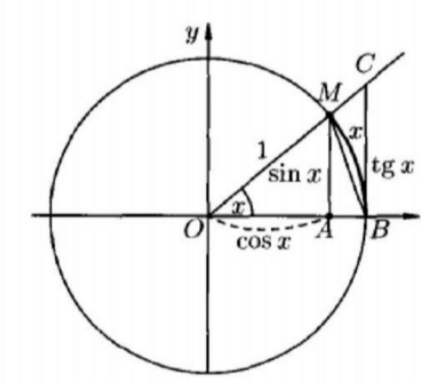
\includegraphics[scale=0.5]{ПервыйЗамечательный.png}}
        \caption{Первый замечательный предел}
        \label{fig:image}
    \end{figure}

    Далее,
    \begin{multline*}
        1-\cos x>1-\frac{\sin x}{x}>0\Leftrightarrow
        2\sin^2\frac{x}{2}>1-\frac{\sin x}{x}>0\Rightarrow\\
        2\cdot\frac{x}{2}>2\sin\frac{x}{2}
        >2\sin^2\frac{x}{2}>1-\frac{\sin x}{x}>0
        \Rightarrow\left|\frac{\sin x}{x}-1\right|<
        |x|,
    \end{multline*}
    причём последнее неравенство справедливо
    при всех $x\in(-\frac{\pi}{2}, 0)\cup
        (0, \frac{\pi}{2}).$

    Если взять произвольное $\varepsilon>0,$
    то, полагая
    $\delta=\min\left\{\varepsilon,
        \frac{\pi}{2}\right\},$
    получим, что при всех $0<|x|<\delta$ выполнено
    неравенство $\left|\frac{\sin x}{x}-1\right|<
        \varepsilon,$ а это по определению означает, что
    $$
        \lim\limits_{x\rightarrow0}
        \frac{\sin x}{x}=1.
    $$
\end{proof}

\begin{proof}
    1) Пользуясь арифметикой пределов и первым
    замечательным пределом, получим
    $$
        \lim\limits_{x\rightarrow0}
        \frac{\tg x}{x}=\lim\limits_{x\rightarrow0}
        \frac{\sin x}{x\cos x}=\lim\limits_{x\rightarrow0}
        \frac{\sin x}{x}\cdot\lim\limits_{x\rightarrow0}
        \frac{1}{\cos x}=1.
    $$
    2) Найдем предел $\lim\limits_{x\rightarrow0}
        \frac{\arctg x}{x}.$ Для этого сделаем замену
    $t=\arctg x,$ откуда по определению арктангенса
    $\tg t=x.$ Так как $x\rightarrow0,$ то
    $\tg t=\frac{\sin t}{\cos t}\rightarrow0,$
    потому мы можем считать, что $t\rightarrow0$
    (более строгое обоснование будет получено,
    когда мы докажем, что арктангенс непрерывен
    в нуле).
    Таким образом, используя теорему о пределе
    композиции, имеем
    $$
        \lim\limits_{x\rightarrow0}
        \frac{\arctg x}{x}=\lim\limits_{t\rightarrow0}
        \frac{t}{\tg t}=1.
    $$
    3) Аналогично пункту 1 получим
    $$
        \lim\limits_{x\rightarrow0}
        \frac{\arcsin x}{x}=\lim\limits_{t\rightarrow0}
        \frac{t}{\sin t}=1.
    $$
    4) Используя формулы тригонометрии, арифметику
    пределов и первый замечательный предел, имеем
    $$
        \lim\limits_{x\rightarrow0}
        \frac{1-\cos x}{x^2}=\lim\limits_{x\rightarrow0}
        \frac{2\sin^2\frac{x}{2}}{x^2}=
        \frac{1}{2}\lim\limits_{x\rightarrow0}
        \frac{\sin\frac{x}{2}}{\frac{x}{2}}
        \cdot\lim\limits_{x\rightarrow0}
        \frac{\sin\frac{x}{2}}{\frac{x}{2}}=\frac{1}{2}.
    $$
    Отметим, что $\lim\limits_{x\rightarrow0}
        \frac{\sin\frac{x}{2}}{\frac{x}{2}}=1,$ так как
    если положить $y=\frac{x}{2},$ то будут
    выполнены все условия теоремы о пределе
    композиции.
\end{proof}

\newpage
\begin{problem}
Вывод второго замечательного предела. Вычисление пределов
\begin{equation}
    \lim_{x\to0} \frac{\ln(1+x)}{x},\:\lim_{x\to0} \frac{e^x - 1}{x},\:\lim_{x\to0} \frac{(1+x)^\alpha - 1}{x}
\end{equation}
\end{problem}

\begin{proposition}
    \textbf{(Второй замечательный предел).}\\
    1) $\lim\limits_{x\rightarrow\pm\infty}
        \left(1+\frac{1}{x}\right)^x=e;$
    2) $\lim\limits_{x\rightarrow0}
        (1+x)^{\frac{1}{x}}=e.$
\end{proposition}
\begin{proof}
    1) Сначала рассмотрим случай
    $x\rightarrow+\infty.$
    Заметим, что
    $$
        \left(1+\frac{1}{n+1}\right)^n=
        \frac{\left(1+\frac{1}{n+1}\right)^{n+1}}
        {\left(1+\frac{1}{n+1}\right)}\rightarrow e \textrm{ и }
        \left(1+\frac{1}{n}\right)^{n+1}=
        \left(1+\frac{1}{n}\right)^n
        \left(1+\frac{1}{n}\right)\rightarrow e
        \textrm{ при } n\rightarrow+\infty,
    $$
    то есть
    $$
        \forall\varepsilon>0\;\exists\;N_1\in\N:
        \forall\;n>N_1\;\left|\left(1+\frac{1}{n+1}\right)^n
        -e\right|<\varepsilon,
    $$
    а также (при этом же $\varepsilon$)
    $$
        \exists\;N_2\in\N:
        \forall\;n>N_2\;\left|\left(1+\frac{1}{n}\right)^{n+1}
        -e\right|<\varepsilon,
    $$
    поэтому при $N=\max\{N_1,\;N_2\}$
    и при $x>1+N$ мы имеем $[x]>N,$
    а тогда
    $$
        e-\varepsilon
        <\left(1+\frac{1}{[x]+1}\right)^{[x]}
        <\left(1+\frac{1}{x}\right)^{x}
        <\left(1+\frac{1}{[x]}\right)^{[x]+1}
        <e+\varepsilon.
    $$
    Таким образом, мы доказали, что
    $$
        \forall\varepsilon>0\;\exists\;N\in\N:
        \forall\;x>N\;\left|\left(1+\frac{1}{x}\right)^x
        -e\right|<\varepsilon,
    $$
    то есть по определению
    $\lim\limits_{x\rightarrow+\infty}
        \left(1+\frac{1}{x}\right)^x=e.$

    Теперь рассмотрим случай $x\rightarrow-\infty.$
    Положим $y=-x,$ тогда
    $y\rightarrow+\infty,$ и мы можем применить
    теорему о пределе композиции:
    $$
        e=\lim\limits_{y\rightarrow+\infty}
        \left(1+\frac{1}{y-1}\right)^y=
        \lim\limits_{y\rightarrow+\infty}
        \left(\frac{y}{y-1}\right)^y=
        \lim\limits_{y\rightarrow+\infty}
        \left(1-\frac{1}{y}\right)^{-y}=
        \lim\limits_{x\rightarrow-\infty}
        \left(1+\frac{1}{x}\right)^x.
    $$
    Объединяя случаи $x\rightarrow+\infty$
    и $x\rightarrow-\infty,$
    получаем, что
    $\lim\limits_{x\rightarrow\infty}
        \left(1+\frac{1}{x}\right)^x=e.$\\
    2) В этом случае сделаем замену
    $\frac{1}{x}=p.$ Тогда $p\rightarrow\infty$
    и мы снова можем применить теорему о
    пределе композиции
    (см. примеры предыдущей лекции
    лекции):
    $$
        \lim\limits_{x\rightarrow0}
        (1+x)^\frac{1}{x}=
        \lim\limits_{p\rightarrow\infty}
        \left(1+\frac{1}{p}\right)^p=e.
    $$
\end{proof}

begin{example}
1) $\lim\limits_{x\rightarrow0}
\frac{\ln(1+x)}{x}=
\lim\limits_{x\rightarrow0}
\ln\left(1+x\right)^{\frac{1}{x}}=
\ln\lim\limits_{x\rightarrow0}
\left(1+x\right)^{\frac{1}{x}}=\ln e=1.$
Здесь переход к пределу по знаком
логарифма возможен именно в силу
непрерывности логарифма в точке $e.$\\
2) Докажем, что
$\lim\limits_{x\rightarrow0}
\frac{e^x-1}{x}=1.$ Положим $e^x-1=y,$
откуда получим $x=\ln(1+y),$ поэтому
$y\rightarrow0$ и
в силу теоремы о пределе композиции
получаем
$$
\lim\limits_{x\rightarrow0}
\frac{e^x-1}{x}=\lim\limits_{y\rightarrow0}
\frac{y}{\ln(1+y)}=1.
$$
3) Воспользуемся теоремой о пределе
композиции для вычисления предела
$\lim\limits_{x\rightarrow0}
\frac{(1+x)^{\alpha}-1}{x}.$
Имеем:
$$
\lim\limits_{x\rightarrow0}
\frac{(1+x)^{\alpha}-1}{x}=
\lim\limits_{x\rightarrow0}
\frac{e^{\alpha\ln(1+x)}-1}{x}.
$$
Положим $\ln(1+x)=t,$ откуда
получим $x=e^t-1$ и при $x\rightarrow0$
также и $t\rightarrow0.$ Таким образом,
$$
\lim\limits_{x\rightarrow0}
\frac{e^{\alpha\ln(1+x)}-1}{x}=
\lim\limits_{t\rightarrow0}
\frac{e^{\alpha t}-1}{e^t-1}=
\lim\limits_{t\rightarrow0}
\frac{\alpha(e^{\alpha t}-1)/\alpha t}
{(e^t-1)/t}=\frac{\alpha}{1}=\alpha.
$$
\end{example}

\newpage
\begin{problem}
Доказательство критерия Коши существования предела функции.
\end{problem}

\begin{theorem} (\textbf{Критерий Коши.})
    Пусть функция $f$ определена на множестве $E,$
    $a$ -- предельная точка множества $E.$
    Функция $f$ имеет предел в точке $a$
    \textbf{тогда и только тогда}, когда для любого
    числа $\varepsilon>0$ существует такое число
    $\delta>0,$ что для любых чисел $x, y \in E,$
    удовлетворяющих неравенствам $0<|x-a|<\delta,$
    $0<|y-a|<\delta$ выполнено неравенство $|f(x)-
    f(y)|<\varepsilon.$ С помощью кванторов:
    $$\exists \lim\limits_{x\rightarrow a}f(x)\;
    \Leftrightarrow\;\forall \varepsilon > 0\;
    \exists \delta >0 :\;\forall \;x, y \in\;
    \stackrel{\circ}{U}_{\delta}(a) \cap E\;
    |f(x) - f(y)| < \varepsilon.
    $$
    \end{theorem}
    \begin{proof}
    \textbf{Необходимость.}
    Пусть $\lim\limits_{x\rightarrow a}f(x)=A$.
    Тогда по определению
    предела по Коши $\forall\varepsilon>0  \ \exists\delta>0:$
    $\forall x \in E\cap\stackrel{\circ}{U}_{\delta}(a)$
    $|f(x)-A|<\varepsilon/2.$ Если $y \in
    E\cap\stackrel{\circ}{U}_{\delta}(a),$
    то $|f(x) - f(y)| = |f(x) - A + A -
    f(y)| \leq |f(x) - A| + |f(y) - A|
    < \varepsilon/2 + \varepsilon/2=\varepsilon.$
    Необходимость доказана.
    
    \textbf{Достаточность.}
    Пусть последовательность $\{a_n\}_{n=1}^{\infty}$
    такова, что
    $a_n \in E\setminus\{a\}\forall n \in \N,$
    $\lim\limits_{n\rightarrow\infty}a_n=a.$
    Тогда при любом $\delta>0$,
    найдётся такое $N \in \N$, что
    $a_n \in E\cap\stackrel{\circ}{U}_{\delta}(a)$
    при всех $n > N,$ из чего по условию следует, что
    последовательность $\{f(a_n)\}_{n=1}^{\infty}$
    фундаментальна, а тогда существует
    предел этой последовательности.
    Пусть $\lim\limits_{n\rightarrow\infty}f(a_n)=A.$
    
    Рассмотрим теперь другую последовательность,
    $\{b_n\}_{n=1}^{\infty},$
    и пусть для неё также выполнены условия, которым
    удовлетворяет последовательность
    $\{a_n\}_{n=1}^{\infty}.$ Если мы докажем, что
    $\lim\limits_{n\rightarrow\infty}f(b_n)=A,$
    то существование предела функции $f$ в точке
    $a$ будет следовать из определения предела
    по Гейне. Отметим, что последовательность
    $\{a_1, b_1, a_2, b_2, ..., a_n, b_n, ...\}$
    также сходится к числу $a,$ поэтому при любом
    $\delta>0$,
    найдётся такое $N_1 \in \N$, что и
    $a_n,$ и $b_n$ принадлежат множеству
    $E\cap\stackrel{\circ}{U}_{\delta}(a)$
    при всех $n > N_1,$ поэтому последовательность
    $\{f(a_1), f(b_1), f(a_2),
    f(b_2), ..., f(a_n), f(b_n), ...\}$
    фундаментальна, а тогда у неё есть предел.
    Тогда у этой последовательности ровно
    один частичный предел, который и совпадает
    с её пределом. Выше мы доказали, что
    $\lim\limits_{n\rightarrow\infty}f(a_n)=A,$
    то есть подпоследовательность
    последовательности $\{f(a_1), f(b_1), f(a_2),
    f(b_2), ..., f(a_n), f(b_n), \textrm{...}\}$
    сходится к $A.$ Тогда и вся
    эта последовательность сходится к $A,$
    поэтому её подпоследовательность
    $\{f(b_n)\}_{n=1}^{\infty}$ сходится к тому
    же пределу, что и завершает доказательство.
    \end{proof}


\newpage
\begin{problem}
Доказательство теоремы Вейерштрасса для монотонных функций. Доказательство свойства $o$-малого (Предложение 1, Лекция 12). Примеры применения асимптотических равенств 1 – 8 и 9 – 13 (два примера).
\end{problem}

\begin{theorem} (\textbf{Теорема Вейерштрасса}).
1) Пусть функция $f$ определена на множестве $E$
и $a$ -- предельная точка
множества $E^-_a.$
Пусть $f$ не убывает и ограничена сверху
на множестве $E^-_a.$ Тогда существует предел слева
функции $f$ в точке $a$ и имеет место равенство
$
\lim\limits_{x\rightarrow a-0}f(x)=
\sup\limits_{x \in E^-_a}f(x).
$\\
2) Пусть функция $f$ не убывает и ограничена
на множестве $E.$ Пусть $a$ -- предельная точка
множества $E^+_a.$ Тогда существует предел справа
функции $f$ в точке $a$ и имеет место равенство
$
\lim\limits_{x\rightarrow a+0}f(x)=
\inf\limits_{x \in E^+_a}f(x).
$
\end{theorem}
\begin{proof}
1) По определению точной верхней грани,
$$\forall\varepsilon>0 \ \exists x_0 \in
E^-_a: M-\varepsilon < f(x_0)\leq M,$$ где
$M:=\sup\limits_{x \in E^-_a}f(x).$
Так как функция $f$ неубывающая, то
$\forall x \in E^-_a: x>x_0$ (что означает,
что $x_0<x<a$ и $x \in E$) выполнены
неравенства $M-\varepsilon<f(x_0)\leq f(x)
\leq M,$ т. е. при любом $\varepsilon>0$
мы нашли такое $\delta:= a-x_0>0,$ что
при всех $x \in E^-_a\cap
\stackrel{\circ}{U}_{\delta}(a)$
выполнено неравенство $|f(x)-M|<\varepsilon,$
т. е. по определению
$$
\lim\limits_{x\rightarrow a-0}f(x)=
\sup\limits_{x \in E^-_a}f(x)=M.
$$
Пункт 2) докажите в качестве упражнения.
\end{proof}

\begin{proposition}
    Запись $f=o(g), \ x\rightarrow a$ равносильна
    также тому,
    что $\lim\limits_{x\rightarrow a}
    \frac{f(x)}{g(x)}=0$
    (при этом считаем, что $g(x)\neq0$
    в некоторой проколотой окрестности
    точки $a$).
    \end{proposition}
    \begin{proof}
    Действительно,
    если $f=o(g), \ x\rightarrow a,$ то
    по определению
    $$
    \lim\limits_{x\rightarrow a}
    \frac{f(x)}{g(x)}=
    \lim\limits_{x\rightarrow a}
    \frac{h(x)g(x)}{g(x)}=
    \lim\limits_{x\rightarrow a}
    h(x)=0,
    $$
    так как $h(x)\rightarrow 0$
    при $x\rightarrow a.$ Обратно,
    если $\lim\limits_{x\rightarrow a}
    \frac{f(x)}{g(x)}=0,$ то функция
    $h:=\frac{f}{g}$ по
    определению является бесконечно малой
    при $x\rightarrow a$,
    а тогда справедливо равенство
    $f(x)=h(x)g(x),$ то есть $f=o(g), \
    g\rightarrow a.$
    \end{proof}